% ++++++++++++++++++++++++++++++++++++++++
% Don't modify this section unless you know what you're doing!
\documentclass[letterpaper,12pt]{article}
\usepackage{tabularx} % extra features for tabular environment
\usepackage{amsmath}  % improve math presentation
\usepackage{graphicx} % takes care of graphic including machinery
\usepackage[margin=0.75in,letterpaper]{geometry} % decreases margins
\usepackage{cite} % takes care of citations
\usepackage[final]{hyperref} % adds hyper links inside the generated pdf file
\usepackage{listings}
\usepackage{csvsimple}
\usepackage{verbatim}
\usepackage{float}
\usepackage{graphicx} % Allows including images
\hypersetup{
	colorlinks=true,       % false: boxed links; true: colored links
	linkcolor=black,        % color of internal links
	citecolor=blue,        % color of links to bibliography
	filecolor=magenta,     % color of file links
	urlcolor=blue         
}
%++++++++++++++++++++++++++++++++++++++++
\setlength{\parindent}{0pt}
\setlength\parskip{1em plus 0.1em minus 0.2em}

\begin{document}
\title{%
PyLab - Radioactive Decay \\
\large PHY224 Lab 2}
\author{Fredrik Dahl Bråten, Pankaj Patil}
\date{\today}
\maketitle
\tableofcontents
\listoffigures
\listoftables

\pagebreak

\section{Exercise 2:  PyLab - Radioactive Decay}

\subsection{Abstract}

In this exercise, we measure and model the rates of emission over time from the radioactive decay of Barium (Ba-137m). 
We have chosen two models, one where the emission rate $I(t) = a*exp(b*t)$, and one where $ln(I(t)) = a*t+b$, 
where a and b are parameters of each model to be fitted to our data, 
$t$ is time, and $ln$ is the natural logarithm. 
After fitting these models to our data, we graphically plot and 
compare these model curves along with the theoretical curve of emission rate, and our data with error bars. 
To evaluate the quality of our models, we calculate and discuss the reduced Chi squared values of our models and data, 
and confirm that the theoretically predicted half-life of Ba-137m lies within the estimated half life with 
uncertainty of our two models. 
This analysis was done in Python by use of the numpy, scipy and matplotlib modules.

\subsection{Introduction}

In this exercise, we measure and model the rates of emission over time caused 
by radioactive decay from a sample of Barium (Ba-137m). 
The corresponding theoretically predicted relationship between emission 
rate ($I$) and time ($t$) is:
$I(t) = I_0*exp(-t/\tau) = I_0 * (1/2)^(t/t_(1/2))$. 
Where $I_0$ is the initial emission rate, $\tau$ is the mean lifetime of the 
isotope, and $t_(1/2)$ is the half-life of the isotope. 
In our experiment, t is the independent variable, and I is our dependent variable.
We are modeling this relationship by using two models, one where the emission rate 
$I(t) = a*exp(b*t)$, and one where $ln(I(t)) = a*t+b$, 
where a and b are parameters of each model to be fitted to our data, 
$t$ is time, and $ln$ is the natural logarithm.

\subsection{Methods, Materials and Experimental Procedure}

We successfully followed the procedures as described in the exercise3.pdf 
document.
The points of data for which we based this analysis on, 
was downloaded from Quercus as instructed by the TAs. 
The uncertainties of the measured data were calculated as described 
in the exercise2.pdf document.

\subsection{Results}

Below in Figure 1 and 2, we see our data from the experiment 
plotted as points with corresponding error bars. 
Furthermore, we see the theoretical curve as described in the introduction, 
along with the curves corresponding to our two models best fitted to our data. 

\begin{figure}[H]
  \centering
  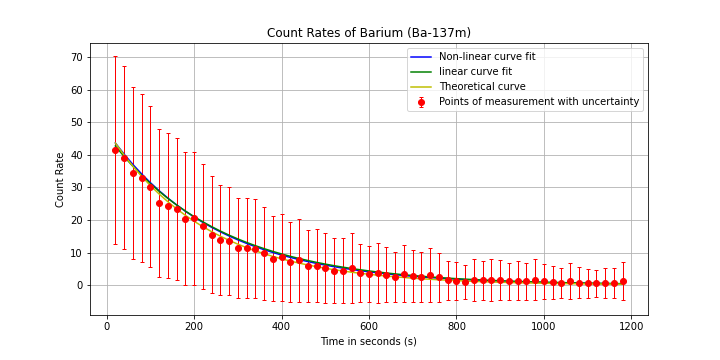
\includegraphics[width=0.95\linewidth]{../Exercise2/Fredrik/Count Rates of Barium (Ba-137m).png}    
  \begin{center}
    \emph{
    Points of measurement with corresponding error bars, theoretical power laws for 
  tungsten and a blackbody, along with our two power law models best fitted to our data 
  points}
  \end{center}
  \caption{Power law, Current vs. Voltage in a Circuit with a Lightbulb}
  \label{power-law}
\end{figure}

\begin{figure}[H]
  \centering
  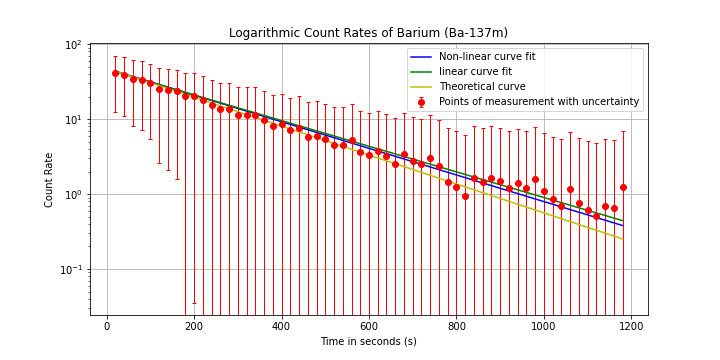
\includegraphics[width=0.95\linewidth]{../Exercise2/Fredrik/Logarithmic Count Rates of Barium (Ba-137m).png}   
  \begin{center}
    \emph{
    Points of measurement with corresponding error bars, theoretical power laws for 
  tungsten and a blackbody, along with our two power law models best fitted to our data 
  points}
  \end{center}
  \caption{Power law, Current vs. Voltage in a Circuit with a Lightbulb}
  \label{power-law}
\end{figure}

The estimated optimal parameters with uncertainty by scipy optimize curve fit are: 
[a,b] = [-0.00393908  3.75408883] +- [0.00090733 0.29589009] for the linear model, and
[a,b] = [ 4.36112915e+01 -4.08767747e-03] +- [1.35411958e+01 1.00398911e-03] for the non linear model.

The reduced Chi squared values for the nonlinear and linear model, respectively, are 0.0069 and 0.0076.
The Half-life of the Barium, predicted by the non-linear model, is: 170.0 +- -42.0 seconds.
The Half-life of the Barium, predicted by the linear model, is: 176.0 +- -41.0 seconds.

\subsection{Discussion}

The reduced Chi squared values we found were very low. This means that our models 
fit our data very well. Thus, the Euclidian distance between the data points and 
our curves is in general very low. However, this is not necessarily a good sign. 
Our reduced Chi squared values should ideally both be equal to one. 
That we have extremely low reduced Chi squared values implies that we do not 
have enough data. It means that we are in risk of overfitting our models to our data.
The non-linear regression method gave a half-life closer to the expected 
half-life of 2.6 minutes = 156 seconds. 170 seconds is closer to 156 seconds, 
than 176 seconds, see half-life results in the Results section. Do however note 
that the theoretical half life falls within both of our models’ estimates of 
the half-lives, with associated uncertainties.
Though it is hard to distinguish the two models in the non-linear plot, in the 
logarithmic, linear plot, you can more easily see that the non-linear model 
returns a curve closer to the theoretical curve than the curve returned by the 
linear model. Both models do however fit the theoretical curve quite well. 
Furthermore, both models are well within the uncertainties of our measurements, 
see Figure 1 and 2 in the Results section.

\subsection{Conclusions}

In this exercise we estimated the emission rate caused by radioactive 
decay of Barium (Ba-137m). We successfully followed the instructions for 
the experiment written in the exercise2.pdf document without issues. 
Though both of our models of emission rate over time returned quite similar 
curves, the non-linear model returned a curve closest to the theoretical curve. 
We have plotted our data with error bars, our models, and the theoretical 
curve in a normal plot, and a plot with logarithmic y-axis. Furthermore, 
we have calculated and discussed each models reduced Chi squared value, 
and confirmed that the theoretical half-life of Ba-137m lies within each of 
our models’ predicted half-lives with uncertainties. 

\pagebreak

\section{Exercise 5:  Random number analysis}

\subsection{Abstract}

\subsection{Introduction}

\subsection{Methods, Materials and Experimental Procedure}

\subsection{Results}

\subsection{Discussion}

\subsection{Conclusions}

\pagebreak

\appendix

\section{Appendix}

\subsection{Data Tables for Exercise 2}
\begin{table}[H]
  \centering
  \verbatiminput{../Exercise2/Fredrik/Barium.txt}
  \caption{Readings of Voltage and Current for 100 $k\Omega$ Resistor}
  \label{100kdata}
\end{table}

\begin{table}[H]
  \centering
  \verbatiminput{../Exercise2/Fredrik/Barium_Background.txt}
  \caption{Readings of Voltage and Current for Potentiometer}
  \label{potentiometerdata}
\end{table}

\subsection{Data Tables for Exercise 3}
\begin{table}[H]
  \centering
  \verbatiminput{../Exercise5/Pankaj/Fiesta_30092021.txt}
  \caption{Readings of Voltage and Current for Exercise 3}
  \label{ex3data}
\end{table}

\begin{table}[H]
  \centering
  \verbatiminput{../Exercise5/Pankaj/Fiesta_Background_30092021.txt}
  \caption{Readings of Voltage and Current for Exercise 3}
  \label{ex3data}
\end{table}

\pagebreak

\subsection{Python Code: Exercise 1}

The Python code for this exercise is divided into two files. Functions.py file contains utility methods
which we will be frequently using in this course. Radioactive Decay.py file contains the code which analyzes
the data.

\subsubsection{Functions.py}
\noindent\rule{\textwidth}{1pt}
\verbatiminput{../Exercise2/Fredrik/Functions.py}
\noindent\rule{\textwidth}{1pt}

\pagebreak

\subsubsection{Radioactive Decay.py}
\noindent\rule{\textwidth}{1pt}
\verbatiminput{../Exercise2/Fredrik/Radioactive Decay.py}
\noindent\rule{\textwidth}{1pt}

\pagebreak
\subsubsection{Program Output}
\noindent\rule{\textwidth}{1pt}
\verbatiminput{../Exercise1/output.txt}
\noindent\rule{\textwidth}{1pt}

\pagebreak

\subsection{Python Code: Exercise 3}

The Python code for this exercise is divided into two files. Functions.py file 
contains utility methods
which we will be frequently using in this course. exercise\_3.py file contains 
the code which analyzes
the data for this experiment.

\subsubsection{Functions.py}

\noindent\rule{\textwidth}{1pt}
\verbatiminput{../Exercise3/Functions.py}
\noindent\rule{\textwidth}{1pt}

\pagebreak

\subsubsection{exercise\_3.py}
\noindent\rule{\textwidth}{1pt}
\verbatiminput{../Exercise3/exercise_3.py}
\noindent\rule{\textwidth}{1pt}
\pagebreak

\begin{thebibliography}{99}

\bibitem{lab-manual-ex2} Lab Manual - PyLab - Ohm and Power laws - Exercise 2.
\bibitem{lab-manual-ex5} Lab Manual - PyLab - Ohm and Power laws - Exercise 5.

\end{thebibliography}

\end{document}
